\documentclass[12pt,a4paper]{ctexart}

\usepackage[top=2.5cm,bottom=2.5cm,left=2cm,right=2cm]{geometry}
\usepackage{graphicx}
\usepackage[table]{xcolor}
\usepackage{booktabs}
\usepackage{multirow}
\usepackage{float}
\usepackage{hyperref}
\usepackage{tabularx}
\usepackage{array}
\usepackage{caption}
\usepackage{enumitem}
\usepackage{amssymb}

\definecolor{greenrate}{HTML}{C6EFCE}
\definecolor{yellowrate}{HTML}{FFEB9C}
\definecolor{redrate}{HTML}{FFC7CE}
\definecolor{headerbg}{HTML}{2F5496}
\definecolor{headerfg}{HTML}{FFFFFF}
\definecolor{grayrow}{HTML}{F2F2F2}

\graphicspath{{images/}}

\hypersetup{colorlinks=true,linkcolor=blue,urlcolor=blue}
\setlength{\tabcolsep}{5pt}

\title{\textbf{阶段性学情分析}}
\author{2026-06-29}
\date{}

\begin{document}
\maketitle
\thispagestyle{empty}
\newpage
\tableofcontents
\newpage

% ============================================================
\section{个人概况}
% ============================================================

\begin{enumerate}[leftmargin=*,itemsep=6pt]
    \item \textbf{个人情况}

    我是跨考生，408科目只在大一学了数据结构，其他三科一点没学过。下定决心考研的时间较晚，大概是清明节后才开始准备考研的。由于刚开始对考研尤其是11408的了解不多，以及需要从大学荒废3年时间后的昏庸状态（三年除了考试没动过笔）调整到学习的状态，导致前期就浪费了很多时间。
    
    这周结课，7月15日考完试，不清楚会不会开展暑期学校之类的（每年政策都在变）。

    \item \textbf{408}

    408是从四月中旬开始的，本来决定直接看王道教材，结果被计组一脚踩死了（正如习题正确率）。然后边看网课，边看王道书，大概20天一本书，推进到现在已经还剩下计网的两章了（也算是追上课程的进度了）。

    之前图进度，计组，操作系统都没有做思维导图，学的也是朦朦胧胧的，到现在还没有一个整体架构。从看了M哥在群里发的怎么学计网那段后，开始计网的时候才开始画导图。

    \item \textbf{数学}
    
    \begin{enumerate}[label=\arabic*.,leftmargin=*]

    \item  数学也是四月中旬开始的，不过当时数学是看同济大学的高数教材（当时完全不知道该怎么学），后来五一假尝试刷了一下题，然后被一脚踩死了。就开始看武忠祥基础篇的书，快速推进，1/2天一章，同步做他的基础严选题（忘了统计，不过记得选择概念题错了挺多的）。

    \item 数一的专项只看了级数，其他都没看，搞完武忠祥基础后觉得基础还是不太行，就准备看张宇的那本书：有必须要去教室的课就看张宇那本书，同时中午不睡觉刷1000题A篇（不过这样持续了两周后，我突然意识到这个好像对下午408影响有点太大了，最开始只是认为计组操作系统本来就难，学着就是会迷糊，结果是困得迷糊，就不推进度去睡觉了），没课就推进线代和概率。1000题A篇只做到了积分学部分，之后的多元微分，二重积分，解微分方程等内容（包括线代和概率）就没做了（计算量高的篇章就会有很多错，觉得不如强化后再来做），这些章节只做了对应的张宇30讲上的例题和课后习题。

    \item 六月中旬开始的高数强化（武忠祥辅导讲义+武忠祥强化课+严选题+880），先做一遍讲义，然后看课，然后做严选题，做880.现在已经开始第三章积分，感觉880，严选题正确率有点低了，选填+解答总的正确率没上80\%（感觉还是掌握的不行）。现在的推进速度大概是9天左右才能完成一章。
    
    \end{enumerate}
    
    \item \textbf{英语}

    英语的推进如下：

    \begin{enumerate}[label=\arabic*.,leftmargin=*]
        \item 不背单词，背其中的红宝书考研词库（顺序版纯折磨，但还是一条路走到了黑）每天100新词输入，背到了3000词左右，开了真题
        \item 一天晚上有时间就做一篇阅读真题（从11开始，估计留个两年的真题模拟，最多隔三天一篇，总体做的一坨，不过也是从之前的通篇看不懂单词，成长到了除了个别单词短语不认识，大概的行文情况还是能搞清的，不过还是做的一坨），然后精读，同时开始使用墨墨背单词里边的真题词库跟着完成的真题背单词，同时不背单词也在每天100新词的输入
        \item 不背单词（红宝书）过完一轮，第二轮每日200新词输入（晚上不太困的话，困了就100个）；墨墨背单词（真题词汇）过完一轮，第二轮每日200新词+复习，但是真题才到2016年
    \end{enumerate}

    \item \textbf{政治}

    买了两个小程序（苍盾+南山，看着一块钱就都买了）
    
    \item 问题
    \begin{enumerate}
    	\item	目前数学强化每个章节是不是太慢了？不过我翻看了目录，前三章页数最多，可能中间的某些章节会快很多，但我还是想要参考一下您的建议。
    	
    	\item	现在我还没学过数一专项，其是否会拖慢很多的进度（有点焦虑）？
    	
    	\item	我觉得我的408选择题（王道）的正确会不会有点低了，其中王道自编题会看这书做，真题自己做，但是总体正确率80\%以下，有的篇章甚至50\%多。（习题完成情况在下一页）
    	
    	\item	我感觉现在我不会做笔记了，也不知道该怎么形容，可能是拖延症？做了880，严选题后，有了没理解的知识点，虽然我会查，会问ai，但是总想着这三章极限，微分，积分是一体的，等到了这三章完了再一起总结，但我害怕这是拖延症的前兆。
    \end{enumerate}
    
\end{enumerate}

\newpage

% ============================================================
\section{408 计算机统考}
% ============================================================

\subsection{四科总览}

\begin{figure}[H]
\centering

\includegraphics[width=0.85\textwidth]{408_overview.png}
\caption{四科一刷正确率对比}
\end{figure}

\begin{table}[H]
\centering
\begin{tabular}{lrrrrr}
\rowcolor{headerbg}\textcolor{headerfg}{\textbf{科目}} & \textcolor{headerfg}{\textbf{题量}} & \textcolor{headerfg}{\textbf{正确率}} & \textcolor{headerfg}{\textbf{真题率}} & \textcolor{headerfg}{\textbf{自编率}} & \textcolor{headerfg}{\textbf{状态}} \\
数据结构        & 595 & \cellcolor{greenrate}85.4\% & 83.0\% & 86.3\% & 一刷完成 \\
计算机组成原理  & 592 & 73.8\% & 78.6\% & 71.6\% & 一刷完成 \\
操作系统        & 650 & 74.5\% & 73.5\% & 74.5\% & 一刷完成 \\
\rowcolor{grayrow}计算机网络 & 383 & 80.2\% & 80.6\% & 76.0\% & 进行中 (第4章) \\
\end{tabular}
\caption{四科完成总览（计网数据截至 6/29，6/30 休息）}
\end{table}

\subsection{各科热力图}

\begin{figure}[H]
\centering
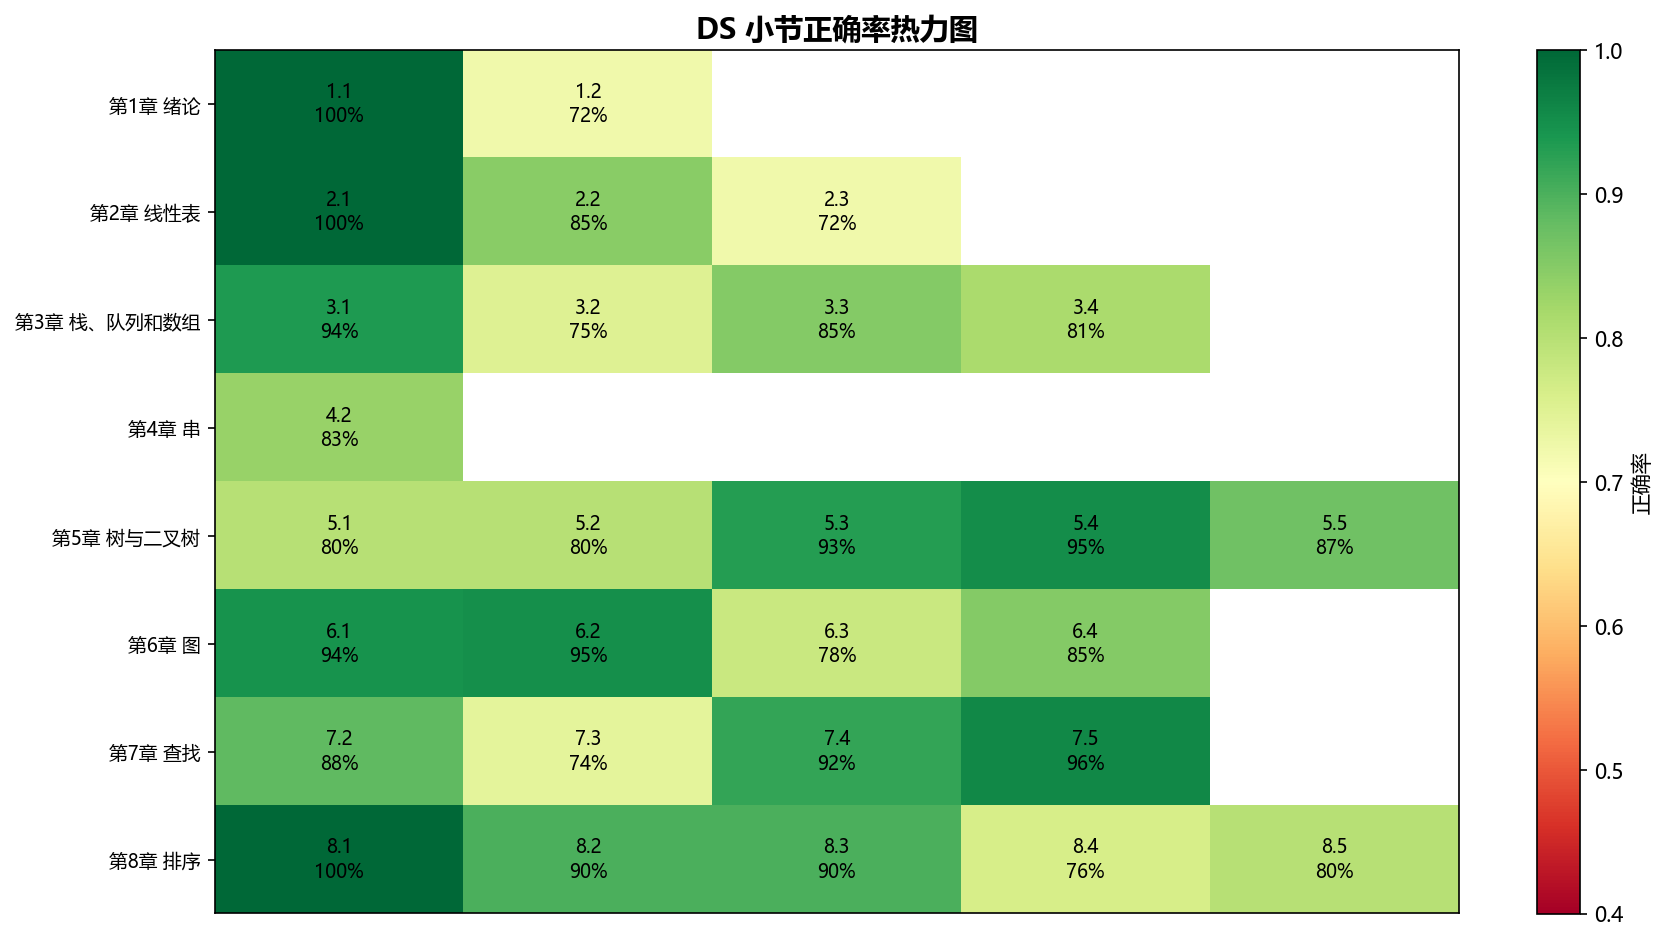
\includegraphics[width=0.48\textwidth]{heatmap_DS.png}\hfill
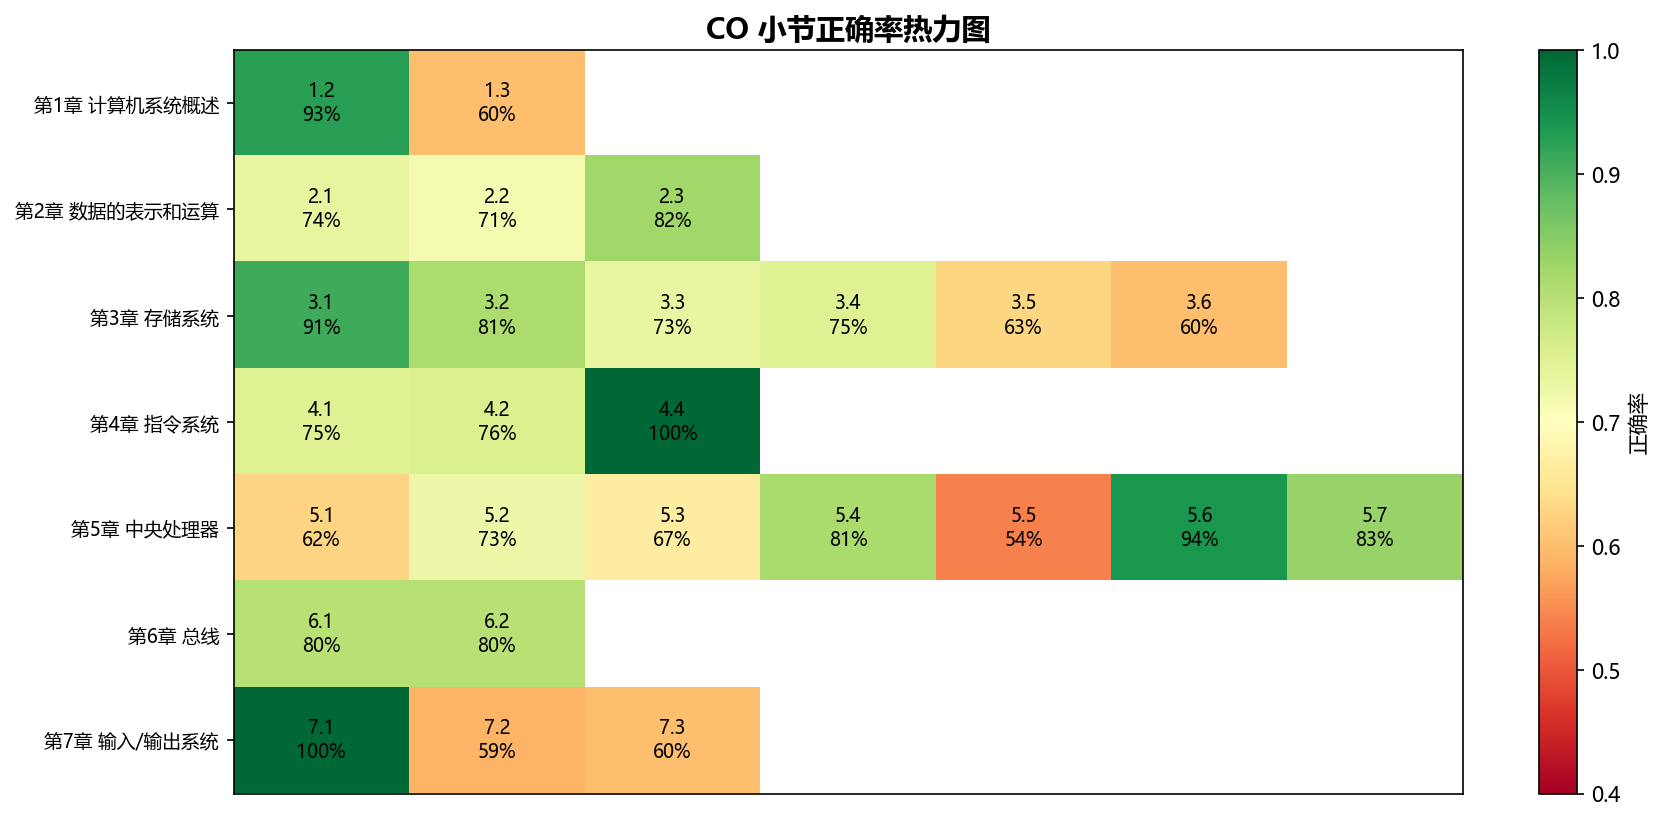
\includegraphics[width=0.48\textwidth]{heatmap_CO.png}
\caption{DS 与 CO 小节正确率热力图}
\end{figure}

\begin{figure}[H]
\centering
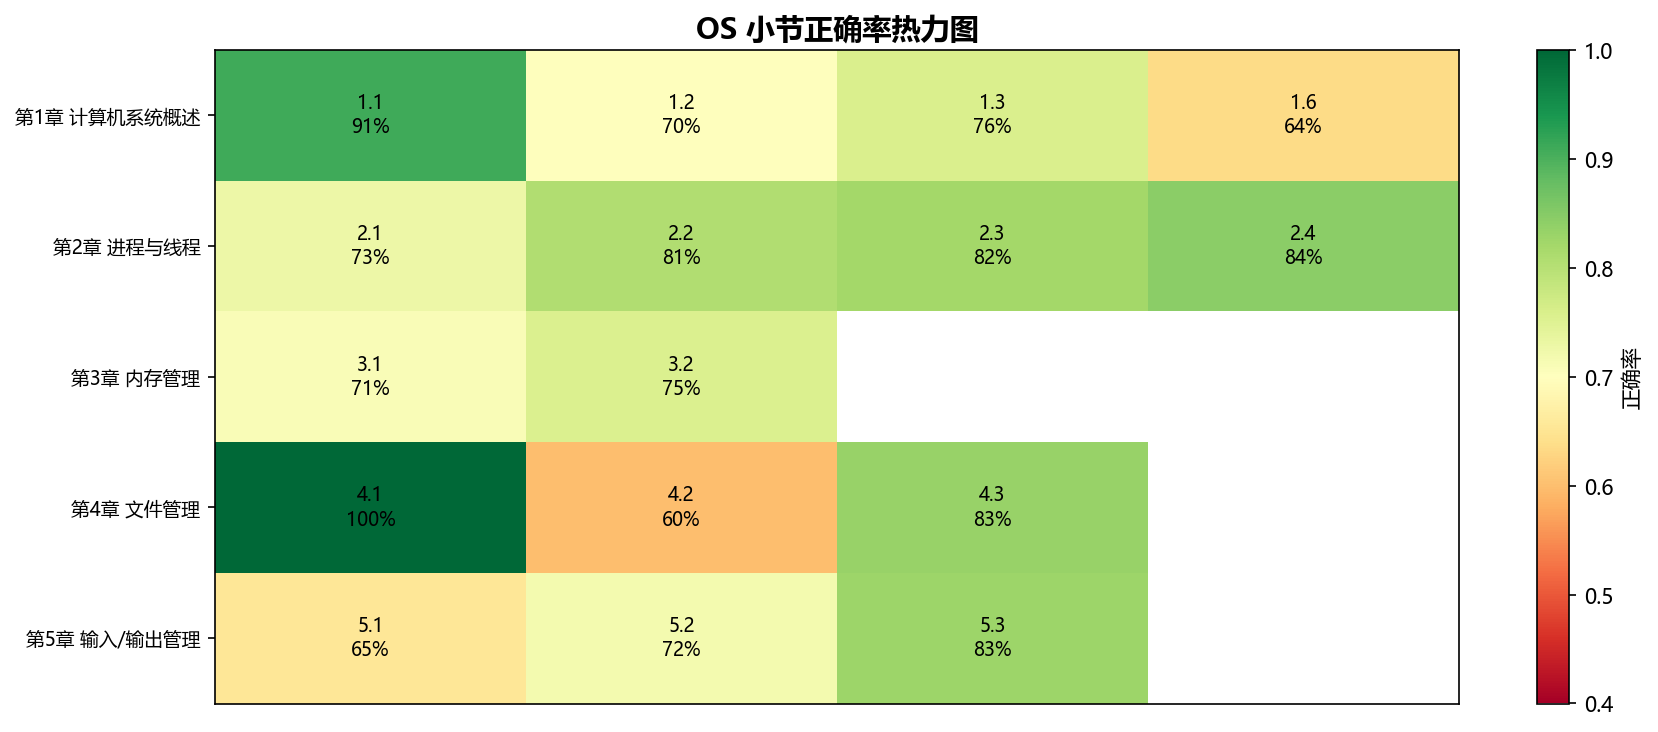
\includegraphics[width=0.48\textwidth]{heatmap_OS.png}\hfill
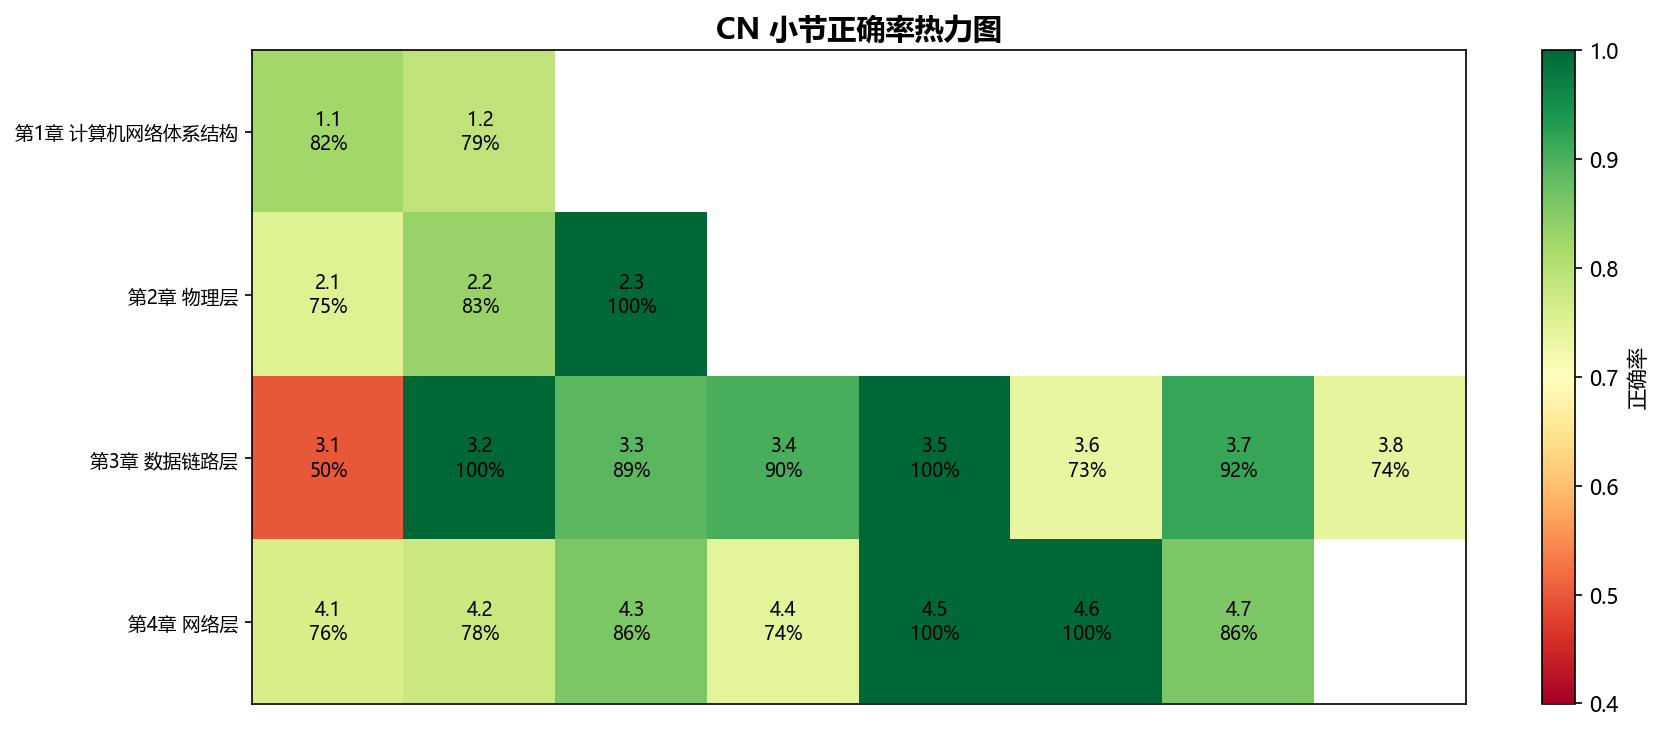
\includegraphics[width=0.48\textwidth]{heatmap_CN.png}
\caption{OS 与 CN 小节正确率热力图}
\end{figure}

\subsection{章节排名}

\begin{figure}[H]
\centering

\includegraphics[width=0.85\textwidth]{408_chapter_ranking.png}
\caption{各章节正确率排名（含四科）}
\end{figure}

\subsection{真题 vs 自编}

\begin{figure}[H]
\centering

\includegraphics[width=0.78\textwidth]{408_zhenti_vs_zibian.png}
\caption{四科真题与自编正确率对比}
\end{figure}

\subsection{薄弱小节}

\begin{figure}[H]
\centering

\includegraphics[width=0.88\textwidth]{408_weak_sections.png}
\caption{正确率最低的 15 个小节}
\end{figure}

\subsection{错题分布}

\begin{figure}[H]
\centering

\includegraphics[width=0.88\textwidth]{408_wrong_count.png}
\caption{错题量最多的 15 个小节}
\end{figure}

\subsection{正确率分布}

\begin{figure}[H]
\centering

\includegraphics[width=\textwidth]{408_distribution.png}
\caption{上：正确率直方图，下：题量-正确率散点图}
\end{figure}

\newpage

% ============================================================
\section{三科薄弱章节}
% ============================================================

\begin{table}[H]
\centering
\begin{tabular}{llp{4cm}p{4cm}}
\rowcolor{headerbg}\textcolor{headerfg}{\textbf{科目}} & \textcolor{headerfg}{\textbf{最弱章}} & \textcolor{headerfg}{\textbf{正确率}} & \textcolor{headerfg}{\textbf{关键薄弱小节}} \\
CO & 第7章 I/O 系统  & 61.8\% & 中断 54\%, I/O 接口 59\%, DMA 60\% \\
   & 第3章 存储系统 & 72\%   & Cache 63\%, 虚拟存储 60\% \\
OS & 第4章 文件管理  & 66.7\% & 目录/文件 60\%, I/O 概述 65\% \\
DS & ---             & ---    & 无低于 70\% 的小节 \\
\end{tabular}
\caption{三科薄弱章节汇总}
\end{table}

% ============================================================
\section{数学强化进度}
% ============================================================

\begin{table}[H]
\centering
\begin{tabular}{lccccccc}
\rowcolor{headerbg}\textcolor{headerfg}{\multirow{2}{*}{\textbf{章节}}} & \multicolumn{3}{c}{\textcolor{headerfg}{\textbf{严选题}}} & \multicolumn{2}{c}{\textcolor{headerfg}{\textbf{880 选填}}} & \multicolumn{2}{c}{\textcolor{headerfg}{\textbf{880 解答}}} \\
\rowcolor{headerbg} & \textcolor{headerfg}{\textbf{选择}} & \textcolor{headerfg}{\textbf{填空}} & \textcolor{headerfg}{\textbf{问答}} & \textcolor{headerfg}{\textbf{率}} & \textcolor{headerfg}{\textbf{日期}} & \textcolor{headerfg}{\textbf{率}} & \textcolor{headerfg}{\textbf{日期}} \\
1. 函数极限连续 & 77.8\% & 100\% & 91.3\% & 94.6\% & 6/18 & 64.7\% & 6/18 \\
2. 一元微分学   & 82.4\% & 90.9\% & 57.7\% & 85.5\% & 6/26 & 65.7\% & 6/25 \\
3--9 章         & --- & --- & --- & --- & --- & --- & --- \\
\midrule
线代 (10--15)  & --- & --- & --- & --- & --- & --- & --- \\
概率 (16--23)  & --- & --- & --- & --- & --- & --- & --- \\
\end{tabular}
\caption{数学强化当前进度}
\end{table}

\end{document}
